\documentclass[8pt]{article}
\usepackage[UTF8]{ctex}
\usepackage[a4paper]{geometry}

\usepackage{amsthm,amsmath,amssymb}
\usepackage{graphicx}
\usepackage{subfigure}
\usepackage{amsmath}
\usepackage{tabularx}
\usepackage{color}
\usepackage{hyperref}
\usepackage{ulem}
\usepackage{multirow}
\usepackage[cache=false]{minted}
\hypersetup{
	colorlinks=true,
	linkcolor=blue
}

\usepackage{appendix}
\geometry{a4paper,centering,scale=0.8}
\geometry{left=2.0cm, right=2.0cm, top=2.5cm, bottom=2.5cm}
\usepackage[format=hang,font=small,textfont=it]{caption}
\usepackage[nottoc]{tocbibind}

\usepackage{algorithm}
\usepackage{algorithmicx}
\usepackage{algpseudocode}
\usepackage{amssymb}
\usepackage{extarrows}
\usepackage{qcircuit}
\usepackage{fancyhdr}
\usepackage{cleveref}

\usepackage{tikz}  
\usetikzlibrary{arrows.meta}%画箭头用的包

\makeatletter
\def\@maketitle{%
	\newpage
	\begin{center}%
		\let \footnote \thanks
		{\LARGE \@title \par}%
		\vskip 1.5em%
		{\large
			\lineskip .5em%
			\begin{tabular}[t]{c}%
				\@author
			\end{tabular}\par}%
		\vskip 1em%
		{\large \@date}%
	\end{center}%
	\par
	\vskip 1.5em}
\makeatother

\newtheoremstyle{compact}%
{3pt}{3pt}%
{}{}%
{\bfseries}{\textcolor{red}{.}}%  % Note that final punctuation is omitted.
{.5em}{\mbox{\textcolor{red}{\thmname{#1}\thmnumber{ #2}}\thmnote{ (\textcolor{blue}{#3})}}}
\theoremstyle{compact}
\newtheorem{innercustomgeneric}{\customgenericname}
\providecommand{\customgenericname}{}
\newcommand{\newcustomtheorem}[2]{%
	\newenvironment{#1}[1]
	{%
		\renewcommand\customgenericname{#2}%
		\renewcommand\theinnercustomgeneric{##1}%
		\innercustomgeneric
	}
	{\endinnercustomgeneric}
}

\DeclareMathOperator{\card}{card}

\newtheorem{theorem}{定理}
\newtheorem{lemma}{引理}
\newtheorem{definition}{定义}
\newtheorem{proposition}{命题}
\newtheorem{corollary}{推论}
\newtheorem{example}{例}
\newtheorem{claim}{声明}
\newtheorem{remark}{注}
\newtheorem{thesis}{论点}
\newtheorem{Proof}{证明}

\def\obj#1{\textbf{\uline{#1}}}
\def\num#1{\textnormal{\textbf{\mbox{\textcolor{blue}{(#1)}}}}}
\def\le{\leqslant}
\def\ge{\geqslant}
\def\im{\text{im }}
\def\P#1{\mathbb{P}\left({#1}\right)}
\def\e{\mathrm{e}}
\def\E#1{\mathbb{E}\left[{#1}\right]}
\def\Var#1{\text{Var}\left[{#1}\right]}


\title{\heiti\zihao{2} 算分第六次作业}
\author{\kaishu\zihao{-3} 周书予\\2000013060@stu.pku.edu.cn}

\CTEXoptions[today=old]
\date{\today}

\usepackage{totpages}
\begin{document}


\fancypagestyle{plain}{
	\fancyhf{}
	\lhead{算法设计与分析实验班}
	\chead{2022 Spring}
	\rhead{第六次作业}
	\cfoot{第 \thepage 页, 共 \pageref{TotPages} 页}
}
\pagestyle{plain}

\crefname{theorem}{定理}{定理}
\crefname{lemma}{引理}{引理}
\crefname{figure}{图}{图}
\crefname{table}{表}{表}	
\maketitle
\section{写出下列问题的线性规划表达}
\subsection*{(a)}
设 $\vec y = (y_1, y_2, \cdots, y_n)^{\text T}$.
\begin{equation*}
	\begin{split}
		\text{minimize} \quad & y_1 + y_2 + \cdots + y_n \\
		\text{s.t.} \quad & \vec{y} \ge \vec{x}\\
		& \vec{y} \ge -\vec{x}\\
		& A\vec{x} \le \vec b + 1\\
		& A\vec{x} \ge \vec b - 1 
	\end{split}
\end{equation*}
\subsection*{(b)}
设 $\vec y = (y_1, y_2, \cdots, y_m)^{\text T}$.
\begin{equation*}
	\begin{split}
		\text{minimize} \quad & y_1 + y_2 + \cdots + y_m \\
		\text{s.t.} \quad& \vec y \ge A\vec x + \vec b\\
		&\vec y \ge 0
	\end{split}
\end{equation*}

\section{教材习题 6.6}
\subsection*{(1)}
\begin{center}
	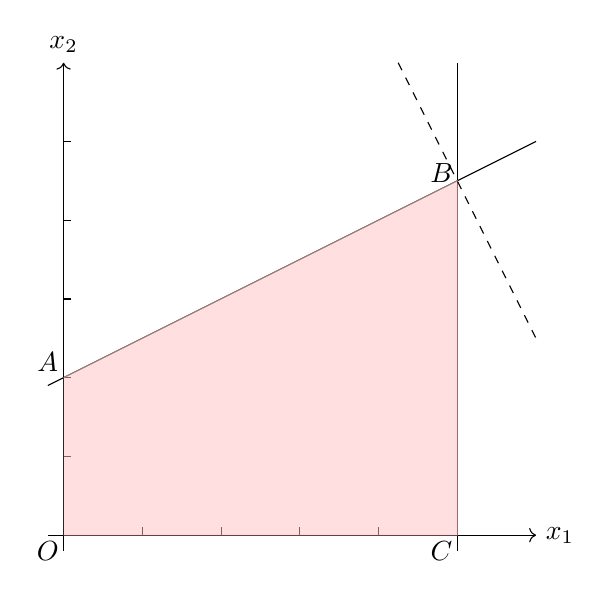
\begin{tikzpicture}[scale=1]
		\draw[->](-0.2, 0) -- (6, 0) node[right]{$x_1$};
		\draw[->](0, -0.2) -- (0, 6) node[above]{$x_2$};
		\draw (5, -0.2) -- (5, 6);
		\draw (-0.2, 1.9) -- (6, 5);
		\node at (-0.2, -0.2) {$O$};
		\node at (-0.2, 2.2) {$A$};
		\node at (4.8, 4.6) {$B$};
		\node at (4.8, -0.2) {$C$};

		\foreach \i  in {1, 2, 3, 4, 5} {
			\draw (\i, 0) -- (\i, 0.1);
			\draw (0, \i) -- (0.1, \i);
		}
		\filldraw[pink, opacity=0.5](0, 0) -- (5, 0) -- (5, 4.5) -- (0, 2);
		\draw[dashed] (4.25, 6) -- (6, 2.5);
	\end{tikzpicture}
\end{center}
最优解在 $B$ 点: $x_1 = 5, x_2 = 4.5$, 最优值为 $14.5$.
\subsection*{(2)}
标准型为
\begin{equation*}
	\begin{split}
		\text{minimize} \quad & -2x_1 - x_2\\
		\text{s.t.} \quad& -x_1 + 2x_2 + x_3 = 4\\
		& x_1 + x_4 = 5\\
		& x_j \ge 0 \ (j = 1, 2, 3, 4)\\
		A = \begin{pmatrix}
			-1 & 2 & 1 & 0\\
			1 & 0 & 0 & 1
		\end{pmatrix}
	\end{split}
\end{equation*}

\begin{itemize}
	\item 取 $B = (P_1, P_2)$, 则 $\begin{pmatrix}-1 & 2 \\ 1 & 0\end{pmatrix} \begin{pmatrix} x_1 \\ x_2 \end{pmatrix} = \begin{pmatrix} 4 \\ 5\end{pmatrix} \Rightarrow \begin{pmatrix} x_1 \\ x_2\end{pmatrix} = \begin{pmatrix} 5 \\ 4.5 \end{pmatrix} \Rightarrow (x_1, x_2) = (5, 4.5)$, 对应点 $B$, 是可行解.
	\item 取 $B = (P_1, P_3)$, 则 $\begin{pmatrix}-1 & 1 \\ 1 & 0\end{pmatrix} \begin{pmatrix} x_1 \\ x_3 \end{pmatrix} = \begin{pmatrix} 4 \\ 5\end{pmatrix} \Rightarrow \begin{pmatrix} x_1 \\ x_3\end{pmatrix} = \begin{pmatrix} 5 \\ 9 \end{pmatrix} \Rightarrow (x_1, x_2) = (5, 0)$, 对应点 $C$, 是可行解.
	\item 取 $B = (P_1, P_4)$, 则 $\begin{pmatrix}-1 & 0 \\ 1 & 1\end{pmatrix} \begin{pmatrix} x_1 \\ x_4 \end{pmatrix} = \begin{pmatrix} 4 \\ 5\end{pmatrix} \Rightarrow \begin{pmatrix} x_1 \\ x_4\end{pmatrix} = \begin{pmatrix} -4 \\ 9 \end{pmatrix} \Rightarrow (x_1, x_2) = (-4, 0)$, 不是可行解.
	\item $P_2, P_3$ 线性相关, 故不能取 $B = (P_2, P_3)$.
	\item 取 $B = (P_2, P_4)$, 则 $\begin{pmatrix}2 & 0 \\ 0 & 1\end{pmatrix} \begin{pmatrix} x_2 \\ x_4 \end{pmatrix} = \begin{pmatrix} 4 \\ 5\end{pmatrix} \Rightarrow \begin{pmatrix} x_2 \\ x_4\end{pmatrix} = \begin{pmatrix} 2 \\ 5 \end{pmatrix} \Rightarrow (x_1, x_2) = (0, 2)$, 对应点 $A$, 是可行解.
	\item 取 $B = (P_3, P_4)$, 则 $\begin{pmatrix}1 & 0 \\ 0 & 1\end{pmatrix} \begin{pmatrix} x_3 \\ x_4 \end{pmatrix} = \begin{pmatrix} 4 \\ 5\end{pmatrix} \Rightarrow \begin{pmatrix} x_3 \\ x_4\end{pmatrix} = \begin{pmatrix} 4 \\ 5 \end{pmatrix} \Rightarrow (x_1, x_2) = (0, 0)$, 对应点 $O$, 是可行解.
\end{itemize}

\section{对偶线性规划}
原线性规划问题可以写成
\begin{equation*}
	\begin{split}
		\text{minimize} \quad & \vec c^{\text T}\vec x \\
		\text{s.t.} \quad& A\vec x \ge \vec b\\
		& \vec x \ge 0
	\end{split}
\end{equation*}
其中 $A = \begin{pmatrix}
	1 & 2 & 3 & 1\\
	2 & -1 & 1 & -3
\end{pmatrix}, \vec b = (2, -3)^{\text T}, \vec c = (2, 3, 5, 6)^{\text T}, \vec x = (x_1, x_2, x_3, x_4)^{\text T}$. 其对偶问题为
\begin{equation*}
	\begin{split}
		\text{maximize} \quad & \vec b^{\text T}\vec y \\
		\text{s.t.} \quad& A^{\text T}\vec y \le \vec c\\
		& \vec y \ge 0
	\end{split}
\end{equation*}
其中 $\vec y = (y_1, y_2)^{\text T}$. 可以展开写为
\begin{equation*}
	\begin{split}
		\text{maximize} \quad & 2y_1 - 3y_2 \\
		\text{s.t.} \quad& y_1 + 2y_2 \le 2\\
		& 2y_1 - y_2 \le 3\\
		& 3y_1 + y_2 \le 5\\
		& y_1 - 3y_2 \le 6\\
		& y_1, y_2, y_3, y_4 \ge 0
	\end{split}
\end{equation*}
\begin{center}
	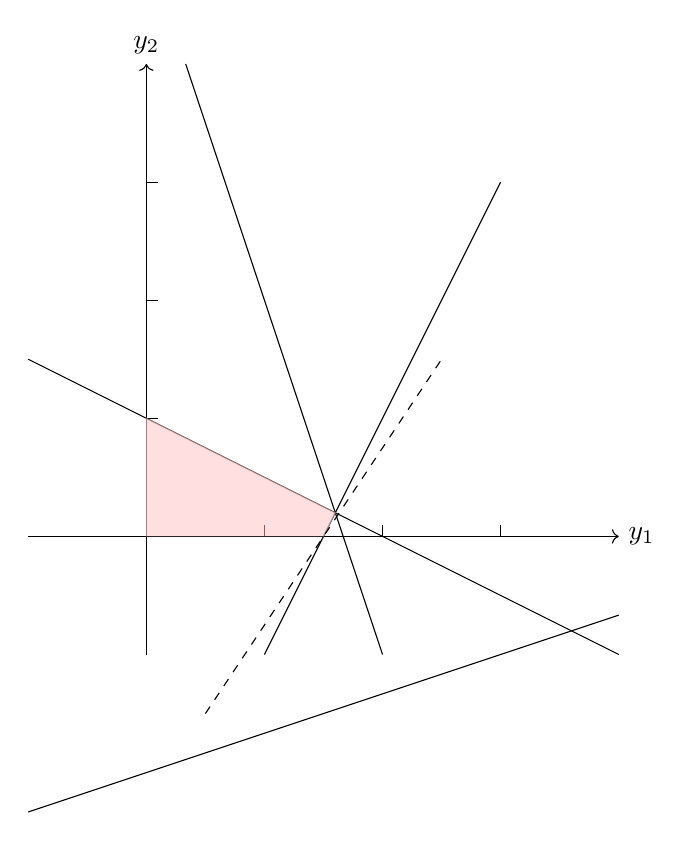
\begin{tikzpicture}[scale=1.5]
		\draw[->](-1, 0) -- (4, 0) node[right]{$y_1$};
		\draw[->](0, -1) -- (0, 4) node[above]{$y_2$};

		\draw (-1, 1.5) -- (4, -1);
		\draw (1, -1) -- (3, 3);
		\draw (1/3, 4) -- (2, -1);
		\draw (-1, -7/3) -- (4, -2/3);

		\foreach \i  in {1, 2, 3} {
			\draw (\i, 0) -- (\i, 0.1);
			\draw (0, \i) -- (0.1, \i);
		}

		\filldraw[pink, opacity=0.5](0, 0) -- (0, 1) -- (1.6, 0.2) -- (1.5, 0);
		\draw[dashed] (0.5, -1.5) -- (2.5, 1.5);
	\end{tikzpicture}
\end{center}

最优解为 $y_1 = 1.5, y_2 = 0$, 最优值为 $3$.

注意到在 $(1.5, 0)$ 处, 对偶问题只有第二个限制条件是紧的, 根据互补松弛型, 原问题的最优解一定形如 $\vec x = (0, x_2, 0, 0)^{\text T}$, 故不难发现最优解为 $(0, 1, 0, 0)^{\text T}$, 最优值为 $3$.

\section{线性规划建模}

我们希望能找到 $\alpha \in \mathbb R^n$, 使得 $\{\alpha^{\text T}\vec x | \vec x \in \mathcal P_1\}$ 与 $\{\alpha^{\text T}\vec x | \vec x \in \mathcal P_2\}$ 不交. 可以考虑最大化 $\min \{\alpha^{\text T}\vec x | \vec x \in \mathcal P_1\}$ 与 $\max\{\alpha^{\text T}\vec x | \vec x \in \mathcal P_2\}$ 的差来实现这一点(不难证明 $\mathcal P_1, \mathcal P_2$ 是闭集, 因此 $\max, \min$ 是良定的).
\begin{equation*}
	\begin{split}
		\text{maximize}_{\alpha} \quad \text{minimize}_{\vec{x}_1, \vec{x}_2} \quad & \alpha^{\text T}(\vec{x}_1 - \vec{x}_2) \\
		\text{s.t.} \quad & A\vec{x}_1 \le \vec b\\
		& C\vec{x}_2 \le \vec d \\
	\end{split}
\end{equation*}

考虑把该问题转换成线性规划问题. 固定 $\alpha$ 时, 该问题是一个关于 $\vec x_1, \vec x_2$ 的线性规划问题, 考虑其对偶型, 可知如下规划问题与原问题等价:
\begin{equation*}
	\begin{split}
		\text{maximize}_{\alpha, \vec y_1, \vec y_2} \quad & -\vec b^{\text T}\vec y_1 - \vec d^{\text T}\vec y_2 \\
		\text{s.t.} \quad & A^{\text T}\vec{y}_1 \ge -\alpha\\
		& C^{\text T}\vec{y}_2 \ge \alpha \\
	\end{split}
\end{equation*}

该问题是一个线性规划问题, 故可以使用线性规划问题求解算法解决. 在解得最优解 $\alpha$ 后, 可以进一步通过解线性规划问题得到 $\min\{\alpha^{\text T}\vec x | \vec x \in \mathcal P_1\}$ 与 $\max\{\alpha^{\text T}\vec x | \vec x \in \mathcal P_2\}$ 的值, 分别记为 $a, b$, 令 $\gamma = \frac{a+b}{2}$, 即可满足 $\forall \vec x \in \mathcal P_1, \alpha^{\text T}\vec x > \gamma, \forall \vec x \in \mathcal P_2, \alpha^{\text T}\vec x < \gamma$.

\end{document}


